\documentclass[10pt,twocolumn,preprint,natbib,authoryear]{sigplanconf}
\bibpunct{[}{]}{,}{a}{}{;}

% force pdflatex to use A4 paper
\setlength{\pdfpagewidth}{210mm}
\setlength{\pdfpageheight}{297mm}
\usepackage{graphicx}
\usepackage{algorithm}
\usepackage{amsmath}

\begin{document}

\conferenceinfo{WXYZ '05}{date, City.} 
\copyrightyear{2005} 
\copyrightdata{[to be supplied]} 

%\titlebanner{Submitted to EuroSys'11}        % These are ignored unless
%\preprintfooter{short description of paper}   % 'preprint' option specified.

\title{Project Voldemort : Batch computed read-only data serving}
%\subtitle{Subtitle Text, if any}

% For double-blind reviewing:
\authorinfo{Roshan Sumbaly}
           {LinkedIn Corp}
           {rsumbaly@linkedin.com}
\authorinfo{Jay Kreps}
           {LinkedIn Corp}
           {jkreps@linkedin.com}
\authorinfo{Sam Shah}
		   {LinkedIn Corp}
           {sashah@linkedin.com}

				
\maketitle

\begin{abstract}
Many internet based companies have started building analytics products backed by computationally intensive data-mining algorithms. One of the important system requirements for these products is the ability to present these results to the end user under strict latency constraints. A good systems practice to achieve this is by decoupling the computation layer from the serving layer. MapReduce paradigm, through the open-source solution Hadoop, has seen a wide spread adoption as the perfect solution for the computation layer. In this paper we present a distributed serving and storage layer called Project Voldemort. We have built and open-sourced this fault-tolerant layer with the ability to serve both read-write and read-only batch computed data. In this paper we will focus primarily on the batch data serving cycle and talk about how it has helped LinkedIn serve multiple TBs of data regularly. With its very simple key-value based interface Voldemort today powers most of our social recommendation products. 
\end{abstract}

\category{D.4.2}{Operating Systems}{Storage Management}
\category{H.3.3}{Information Search and Retrieval}{Information Storage}
\category{H.3.3}{Information Search and Retrieval}{Information Search and Retrieval}

\terms
Design, Performance

\keywords
database, low latency, distributed, offline

\section{Introduction}
The product data cycle of a typical consumer web company consists of a continuous cycle of three phases - data collection, processing and finally serving. The data collection phase deals with gathering raw events like user activity, shares, etc. from various storage solutions as well as logging systems. The ability to horizontally scale with the increase in number of data sources is a tough problem and has been solved in the form of various distributed log aggregation systems. Some examples of these include LinkedIn's Kafka\cite{1}, Facebook's Scribe\cite{2} and Cloudera's Flume\cite{3}. Besides providing access to numerous data-sources these systems also provide pluggable sink interfaces, in particular the ability to push the data into batch processing systems like the Hadoop ecosystem ( in particular HDFS )\cite{4}. The Hadoop ecosystem then in-turn provides a diverse offering of query languages thereby providing the ability to run complex product driven algorithms as batch jobs. The size of the output generated by these jobs can end up being massive. For example in the context of social networks most algorithms tend to derive relationships between items ( where items could be users or any other important facet ). This sparse relationship data can get really huge when dealing with millions of items. The end goal of most of this processing is to surface insights which can then be provided back to the user.

In this paper we talk about our solution for the last phase of this cycle, called Project Voldemort, and how it fits into our product ecosystem. We've built this serving platform with the aim to quickly update the online index with new offline data and still have minimum latency impact for the live lookups. The tricky part of this system is the efficient movement of large amounts of the data, especially since we have constraints to refresh these `insights' on a daily basis. At LinkedIn our largest cluster deals with multiple TBs of data and regularly pushes around 3 TBs to the site. Another important feature that we wanted to support was the ability to still deliver results under regular failures. We also built the system with horizontally scalability in mind so as to support addition of new products immediately. Voldemort has been running in production at LinkedIn for the past 2 years and has successfully been serving various user-facing features like `People you may know', `LinkedIn Skills' and `Who viewed my profile'. One of the reasons behind its success and quick adoption within the company has been its simple key-value like API which makes it easy to test. This has helped our engineers to quickly iterate and now we have our largest cluster serving around 100 features ( stores ), most of which are serving our 120 million user base.

The rest of the paper has been structured into 5 sections. In Section 2 we talk about some of the existing solutions and how it compares with Voldemort's design. The next section, Section 3,  talks about our system architecture and its evolution. Voldemort is heavily inspired from Amazon's Dynamo\cite{5} and was hence initially designed to only support the fast online read/write load. But its pluggable architecture, in particular the ability to add multiple storage engines, allowed us to build our own custom read-only storage engine and integrate with the offline data cycle. Section 4 goes into details about the read-only storage engine and the various design decisions we made while building it. In Section 6 we give details about our experiences while using Voldemort at LinkedIn. We will also talk more about performance results. We finally discuss future work and conclude in Section 7. 


\section{Related Work}
The most commonly deployed serving system in various companies is MySQL. The two most used storage engines of MySQL - MyISAM and InnoDB - provide bulk loading capabilities into live system with `LOAD DATA INFILE' statement. MyISAM is the better amongst the two because of its compact on-disk space usage and its ability to delay the re-creation of the index to a time after the load\cite{6 - http://dev.mysql.com/doc/refman/5.5/en/optimizing-myisam-bulk-data-loading.html}.  Unfortunately we still have to deal with the problem of needing lots of memory during the re-creation which in turn may affect our live requests performance. MyISAM also provides the ability to build compressed read-only tables \cite{7 - http://dev.mysql.com/doc/refman/5.5/en/myisampack.html} which can increase the speed of loading. Even though this decreases the load time, we still have no way to parallelize loads while also locking the complete table for the duration of the load. Obviously this doesn't work for us since applications at LinkedIn cannot have down-time. 

A lot of work has also been done to add bulk loading ability to some new shared-nothing cluster\cite{The Case for Shared Nothing Database} databases similar to Voldemort. In \cite{8 - Efficient Bulk Insertion into a Distributed Ordered Table} tackles the problem of bulk insertion into range partitioned tables in PNUTS \cite{9 - PNUTS paper} by adding another \emph {planning phase} to gather more statistics for the movement. Another paper from the same team \cite{A Batch of PNUTS: Experiences Connecting Cloud Batch and Serving Systems} shows how they used Hadoop to batch insert data faster into PNUTS.

All of the above approaches try to optimize the performance on the current serving cluster during loads and update the indexes (B-tree in most scenarios ) on the live system. Since we cater to data-sets that completely need to be changed at once the approach that we have adopted builds the full index offline. Using MapReduce for this purpose has been a well researched idea with various systems. For example various search systems, like Katta\cite{10 - Katta link} and \cite{Distributed Indexing for Semantic Search}, have hooks to build their indexes in Hadoop and then pull the indices from HDFS to serve search requests. This idea has also been extended to various databases. Both \cite{11 - Distributed Indexing of Web Scale Datasets for the Cloud} and \cite{Parallel Bulk Insertion for Large-scale Analytics Applications} build HFiles ( equivalent to Google's SSTable file - Persistent and immutable map file ) offline in Hadoop and then ship them over to be consumed immediately by HBase. They bypass the conventional client API which would do something similar to MySQL i.e. first persist to log, buffer in memory and then flush periodically. The same approach has been adopted by Cassandra in its new \emph{sstableloader}\cite{http://www.datastax.com/dev/blog/bulk-loading} functionality. These approaches definitely alleviate the cluster from sudden memory usage pattern changes due to index changes. 

But all of the above solutions don't solve one very important use case of ours. The general development pattern that we've seen for data products is that engineers come up with new algorithm tweaks and then push out the corresponding data changes in steps, while continuously monitoring their metrics. The problem kicks in when a new push of data is resulting in a major drop in metrics. In such a scenario having to run a batch Hadoop job to bulk load new data back in would be very time-consuming. Our novel storage layout tries to solve this problem by providing some form of rollback mechanism. 
 
From an architecture perspective, Voldemort falls into the league of many previous P2P storage systems. There have been various structured DHTs, like Chord and Pastry, which provide O(log N) lookup. We are more inspired by Dynamo and Beehive which tries to decrease the variance in latency due to multi-hop routing by saving more state and providing lookups in O(1). Similar to Dynamo, Voldemort also supports per tuple based replication for availability purposes. Updating all replicas is easy in the read-only batch scenario since these are pre-computed and then pushed over to Voldemort at once. To make replica updates fast in read-write scenario we allow our updates to some of the replicas of a key to be asynchronous. Network partitions or server failures during these asynchronous updates can result in inconsistencies between replicas. To solve this problem we version every replica and then delegate any resolution to the application during the $get$ time. This application level resolution has been inspired by previous work by Bayou\cite{http://www2.parc.com/csl/projects/bayou/pubs/uist-97/Bayou.pdf}. 

\section{System Architecture}

Before we start let us define some of the concepts and terms we will use in this paper. A Voldemort \emph{cluster} can contain multiple \emph{nodes} ( or \emph{servers} ) . Each server has a unique id associated with it. All the nodes in the cluster store the same number of \emph{stores} which correspond to database tables. General usage patterns have shown that a site-facing feature may map to either one store or multiple stores. For example, a feature dealing with group recommendation may map to two stores - one storing member id to recommended group ids and second storing a group id to their corresponding description. Every store has a list of configurable parameters

\begin{itemize}
	\item \emph {Replication factor} - Number of servers onto which each key-value tuple is replicated 
	\item \emph {Required reads} - Number of servers which we read from in parallel during a $get()$ before declaring a success
	\item \emph {Required writes} - Number of server responses we block for before declaring success during a $put()$
	\item \emph {Key/Value serializer and compression} - We can different serialization format for the key and value. Voldemort supports various serialization formats - some of which include Avro, Protocol buffers, Thrift and Custom binary JSON. Also we support per-tuple based compression which can be applied to key and/or value. All these are invoked only on the client side while the server only deals with byte arrays. The exception to this is a relatively new feature called `server side transforms', which has been discussed further below. 
\end{itemize}

\subsection{System components}
  
\begin{center}
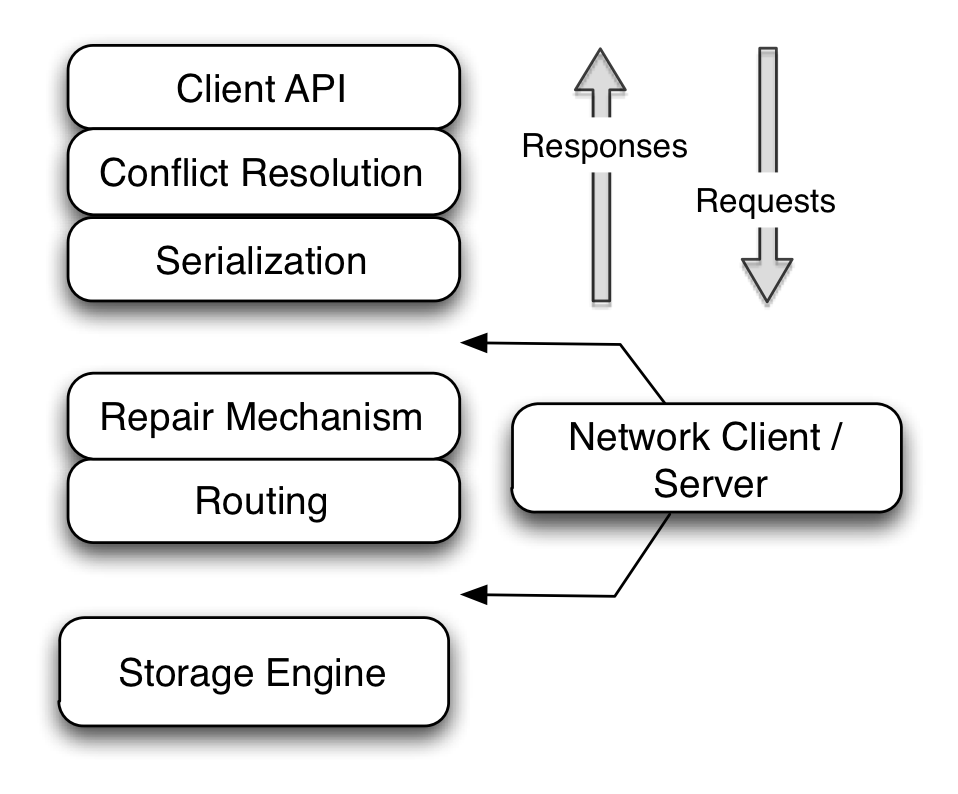
\includegraphics[scale=0.65]{arch.png}
\end{center}

Voldemort has been inspired from Amazon's Dynamo paper and has a similar pluggable architecture. Figure 1 shows the architecture of Voldemort. Each box represents a module, all of which share the same simple interface. Every module has exactly one functionality, which we'll explain in the following sub-sections. This type of layering makes it easy to interchange modules and place them in any order. For example we can have the routing module on either the client side or the server side. Functionality separation at module level also allows us to easily mock these modules for testing purposes. One of the most common uses of this can be found in our unit tests where we mock the storage layer to use an in-memory hash map based engine. 

\subsubsection {Client API }  
Starting from the top our client has a simple $get$ and $put$ API with no support for complex operations like joins, foreign key constraints, etc. Here are the functions that we provide. 
\begin{verbatim}
VectorClock<V> get (K key)
put (K key, VectorClock<V> value)
VectorClock<V> get (K key, T transform)
put (K key, VectorClock<V> value, T transform)
\end{verbatim}

This first two functions are simple except we version every tuple with a vector clock ( more about this in the next sub-section ). The next two functions show a very powerful feature in Voldemort which allows you to run a transform / function on your data when it is on the server side. Correctly using this can help us in saving some network bandwidth by transferring only the required parts of a large value. A common example of this is when we have a list of entities as the value. We can then run a transformed $get$ to only retrieve a sub-list or a transformed $put$ to append an entity to your list. 

\subsubsection {Routing layer }  
Before we talk about conflict resolution it is important we understand how routing and replica assignment works. Since Voldemort can be thought of as a massive hash table we need a way to partition the data across the multiple servers. The best partitioning implementation would be one which would split the `hot' set of data into minute chunks and spread them across such that they fit in memory on the individual servers. Also server failures, maintenance or just being overloaded are common scenarios. In such cases we definitely don't want our clients to stop serving data. This motivates the need to also replicate the data onto multiple servers. 

The Dynamo paper solved these problem by using `virtual nodes' along with consistent hashing. The initial approach they took was to visualize the integer hash values as a ring beginning at 0 and circling around to max value ( in case of MD5, 128 bits = 2$^{128}$-1 ). Then each node is assigned an integer which is in turn hashed ( using MD5 ) into this ring multiple times ( each location of it is called a token ). Then each node becomes responsible for the region between its token and the predecessor token ( belonging to another node ) on the ring. A key is assigned to a node by hashing the key to yield its position in the ring and then jumping the ring clockwise to find the first token ( and corresponding node ) with a greater hash value. Similarly the replicas are decided by jumping further till you find `replication factor' ( $N$ ) number of tokens belonging to different nodes. This list of nodes is called the `preference list' for the key. This consistent hashing approach has the advantage that if a node goes down the affected keys are only ones hashed to regions close to the tokens belonging to the affected node. The disadvantage is that we may result in unequal key ranges because the uneven hashing of the tokens thereby resulting in a skew. 

To solve this problem the better approach is to instead split the hash ring into equal size `partitions' and then assign these partitions to nodes. To generate the preference list we need to first hash the key to a partition and then continue jumping the ring clockwise till we find $N$-1 other partitions belonging to different nodes. This equal sized range base approach helps solve the imbalanced key range problem. It also indirectly helps in data-management ( as further discussed in Section ) since having segregated logical file groups for a partition can help with rebalancing. 

Since our routing layer is customizable it was easy to plug in another variant of the above consistent hashing algorithm to support routing in multiple data-center environment. For the same we start by grouping nodes into logical clusters that we call `zones'. A zone in the real world can be a data-center, a rack or just a group of nodes close together. Besides this we have a `zone proximity list' which contains information regarding zone distances ( For example, Zone A is closer to Zone B than Zone C ). Now we provide the user the ability to decide how many replicas they want per zone and then while generating the preference list jump the ring to find partitions belonging to different nodes and zones. Once the routing module generates the preference list it reorders it depending on the proximity list of the zone it is present in. This enables us to make sure requests first go to local zones instead of remote zones. 

Following is an example of how the two routing strategies would generate different preference lists for the same key.  


\begin{center}
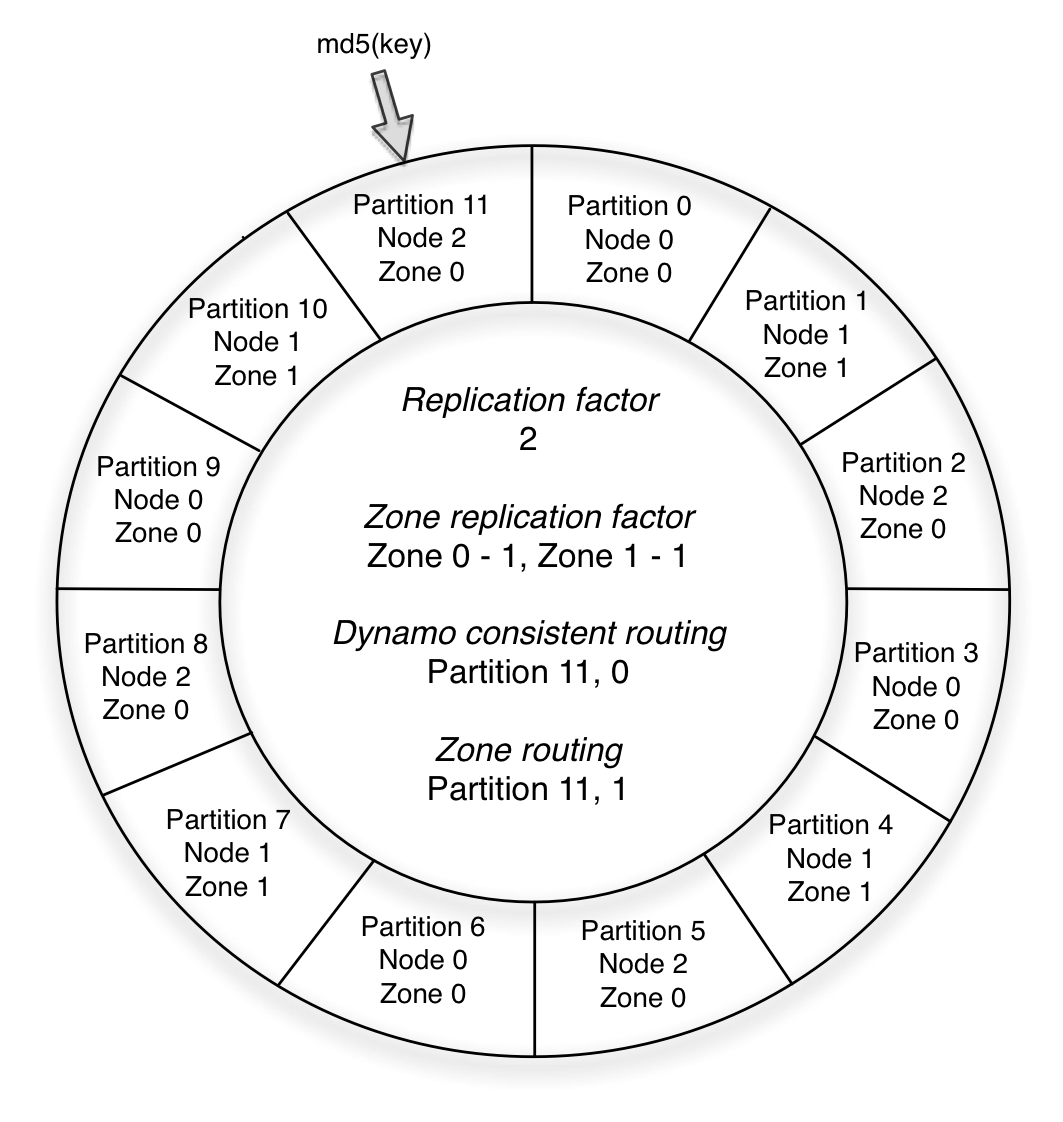
\includegraphics[scale=0.65]{hash.png}
\end{center}

\subsubsection {Conflict Resolution } 
In distributed systems network partitions are common. In such scenarios if you are updating various replicas of the same key it becomes very essential that we have some form of versioning in order to resolve conflicts. In particular these versions should be able to detect overwrites and also allow us to detect conflicts. 

For the same we use the concept of vector clocks \cite{Time, clocks, and the ordering of events in a distributed system}. A vector clock keeps a counter for each writing server, and allows us to calculate when two versions are in conflict and when one version succeeds or precedes another. In practice this is a list of node id and counter pair. These counters are incremented depending on which node acts as the pseudo-master for a request. For example,  $[1:10,2:3]$ signifies that node id 1 was master for this replica 10 times while node id 2 was 3 times. The use of vector clocks allows us to support some form of optimistic locking on the client side. For example, if two clients both try to update the same key with the same vector clock only one of them will succeed while the other will be thrown a special error. This special error can then trigger the client to do the same get() and put() operation again some number of times. We call this `applyUpdate' and have seen its usage in various applications that require a `read, modify, write if no change' loop ( Eg. Counters )

\subsubsection {Consistency Mechanism }

When doing multiple simultaneous writes distributed across multiple servers consistency of data becomes a difficult problem. The traditional solution to this problem is distributed transactions but these tend to have two problems. Firstly they are very slow due to the multiple round trips required for handshakes and acknowledgements. The other problem with them is that they tend to be very fragile and cannot work if some of the servers are down. One solution to this problem is to tolerate the possibility of inconsistency and provide mechanisms of eventually catching up on all the missed updates. 

For the same we provide two consistency mechanisms in Voldemort for read-write stores - read repair and hinted handoff. Read repair method detects these inconsistencies during read-time and resolves the problem by doing asynchronous writes. The only disadvantage of this method is that the user needs to provide some application specific logic to resolve conflicts. The other consistency mechanism, hinted handoff, is triggered during write time. If during a $put()$ we find that some of the destination nodes are down ( and we have  satisfied our `required writes' ) the client triggers an asynchronous write to a special store called `slop store' on one of the live nodes. We write a `hint' to this store - where a hint contains the node id of the down node along with the updated value that it missed. We then have a periodic background job running on every node which tries to push these `hints' out to the down nodes.

\subsubsection {Storage engines}
The storage layer is pluggable with a simple interface which all storage engines must implement. Besides the basic $get()$ and $put()$ functions every storage engine must also implement the following two functions 
\begin{verbatim}
Iterator<K> keys() 
Iterator<Pair<K, VectorClock<V>>> entries()
\end{verbatim}  
This then allows us to provide streaming get interface which can be helpful for debugging as well as rebalancing. The various storage engines that Voldemort supports are Berkeley DB Java Edition, in-memory hash map, MySQL, Krati and our custom read-only storage engine. 

\subsubsection{Administrative service}
Besides running the above stack every node also runs a special service on every node which allow administrators to run special commands. Here we list some of the commands that we support.

\begin{itemize}
	
	\item \emph{Add / delete / truncate store} - Ability to add or delete a store without down time. We can also truncate the complete data without deleting the store completely. 
	\item \emph{Stream data} - We have the ability to stream data out of a store. If the store is read-write, we can stream data in as well. 
	\item \emph{Read-only store operations } - Trigger the batch fetch from Hadoop as well as other related operations. We will discuss this further in Section 4. 
	\item \emph{Slop operations } - Ability to manually trigger the periodic pushing job for hinted handoff. 
	
\end{itemize}

\begin{center}
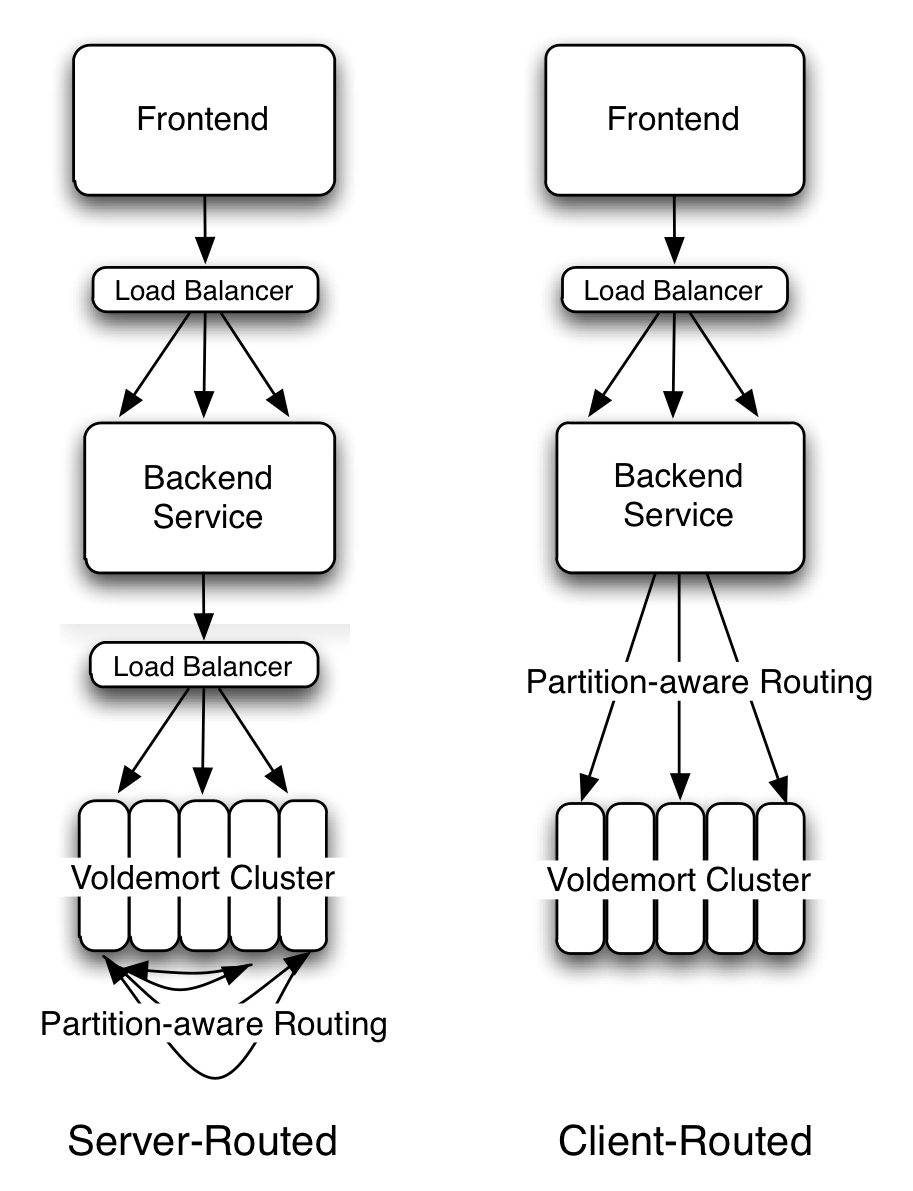
\includegraphics[scale=0.60]{fullstack.png}
\end{center}
	
Now that we know the individual components, let us look at how Voldemort is being used inside the complete LinkedIn stack. As shown in Figure 2 we support both server side as well as client side routing. Client side routing gives us the benefit of having one less hop as the clients now have information about exactly where the replicas for a key are. This is beneficial from a latency as well as throughput aspect since we have less number of services acting as bottlenecks. The disadvantage of client side routing is it makes the client side code-base large because of the extra routing and replication layer. It also makes rebalancing difficult because we now need to update the cluster configuration on all the clients. 

\section{Read-only storage engine}

Before we started writing our own custom storage engine we decided to evaluate all the current storage engines that Voldemort supported in order to see if they could fit our bulk loading use-case. The first two storage engines that we tried were MySQL and Berkeley DB ( BDB ). We started by evaluating the various storage engines provided by MySQL. Our criteria for success was the ability to bulk load data as fast as possible and with minimum disk space overhead. The first simple and most naive way to load data into MySQL is by using multiple `INSERT' statement. The problem with this approach is that every statement results in an incremental change to the underlying index structure ( in this case - B+ tree ) which in turn can result in a lot of disk I/O. To solve this problem, MySQL provides the `LOAD DATA' statement which tries to bulk update the underlying index. The problem here is that we will need to lock the complete table during bulk loads if we use MyISAM storage engine since it supports only table wide lock. This results in all incoming requests being queued and not served during the loading. This problem is solved by InnoDB which supports row-level locking, but comes at the expense of having a huge disk space overhead for every tuple. This can result in a massive increase of data during bulk loads. Unfortunately the only way to get InnoDB to perform as well as MyISAM for bulk loads is by having the special requirement of having your data ordered by primary key.  \cite{http://blogs.oracle.com/carriergrademysql/entry/tips_for_bulk_loading}. 

The general learning from the above tests was that we should aim to build our index offline rather than on the live server. Building the index on the live server can start taking up both CPU and IO resources. We decided to skip InnoDB from future tests due to huge space requirements and tried to build MyISAM storage engine data offline. To do so we leverage the fact that MySQL allows you to copy database files from another node into a live database directory to automatically make it available for serving. We set up a separate cluster where-in we would bulk load and then eventually copy the data over to the list cluster. The biggest problem with this approach is the extra maintenance cost that we need to incur to have a separate MySQL cluster with exactly the same number of nodes as the live one. We also need to write a lot of custom code to deal with failure scenarios during these intermediate bulk pushes. Also the lack of ability to load compressed data directly makes this process more time consuming since now we are copying our data multiple times - once as a flat file to the bulk load cluster, then to the actual database during the LOAD statement and finally the raw data copy to the actual live database. 

One of the biggest problem that the offline system above has is that it doesn't scale well due to its dependency on the redundant MySQL servers. Also this dependency makes the complete process prone to downtime due to failures. What if we could use the inherent fault tolerance and parallelism of Hadoop and instead build individual node / partition level data stores, finally shipping over the data to Voldemort? Also the massive adoption of HDFS as the data `sink' makes it an ideal location to act as our source of data. Most of LinkedIn's data now flows into HDFS through Kafka thereby allowing us to run simple MapReduce programs on top of it. One of the best single node high performance storage engines present today is BDB. Combining BDB and Hadoop, we can try to dump the output of reducers to BDB files, copy it over to HDFS and finally push the final results over to Voldemort. This approach has been tried by ElephantDB \cite{ElephantDB}, but still has the problem of redundant copying from local BDB files to HDFS. This extra copying can be a real bottleneck when we are dealing with TBs of data. 

From the above experiments we came to the conclusion that we required our own custom storage engine. Our new custom storage engine, along with its complete pipeline, should have the following properties. 
\begin{itemize}
\item \emph {No performance impact on live requests}: The incoming requests to the live store should not have any major performance impact during the data load. There is a major tradeoff that we need to worry about during the load. If we are modifying the current index on the live server then we want to finish the bulk load as fast as possible. But pushing the limit on the bulk load can result in an increase of I/O which can then hurt performance. This motivates us to not touch the live index at all and completely rebuild it offline. 
\item \emph {Fault tolerance and scalability at every step }: Every step of this data push pipeline should be able to handle failures. We aim to use Hadoop as our computation layer for building the index. Inherent fault tolerance in Hadoop allows us to run index generation on massive datasets without worrying about failures. Similarly we finally intend to store our data in HDFS whose replication provides us availability. Finally Voldemort as the serving layer is an ideal fit since our routing strategies allow us to fall back on replicas in case of failures. All of these systems are also able to scale horizontally due to already existing support for expansion without downtime. 
\item \emph{Rollback}: The general trend that we see at LinkedIn is that data is being treated more like code. This means we can definitely have bad data which may have been generated due to a bad new algorithm or some missing source data. Introduction of bugs in code are fixed in two ways - quick bug fix or rollback of code to a good state. For the bug fix we would need to re-compute the complete data-set and push it again. Since this process can take a really long time it would be better if our storage engine could instead support quick rollbacks by storing the previous data-sets. This also requires us to be then pushing complete data-set every time. 
\end{itemize}

We have kept the above desired properties in mind and built a completely new data pipeline. This pipeline first consists of a new storage engine for Voldemort which is easy to build in Hadoop ( Section 4.1 ). We then explain the versioning of data and how it can help to satisfy the rollback criteria ( Section 4.2 ). We finally conclude by explaining how it fits into the complete data deployment cycle along with some real world production scenarios and how we dealt with it. 


\subsection{Storage format}

A quick study of previous literature showed that most storage formats try to build data structures that keep the data memory-resident in the process address space. Unfortunately most of them do not think too much about caching being done by the operating system's page cache. Classical example of this is InnoDB storage engine of MySQL which buffers both key and data pages resulting in double caching \cite{Page 203 - Understanding MySQL internals} at both OS as well as MySQL level. The latency gap between access from page cache vs disk is so massive that the only real performance benefit would be for elements already in the page cache. In fact now this custom structure may even start taking memory away from the page cache. This motivated us to build our storage engine to exploit the page cache instead of maintaining our own complex data structure. Since our data is immutable the simplest way to do so is by memory mapping the entire index into the address space. Since Voldemort has been written in Java and runs on the JVM, delegating the memory management to the operating system is also a big plus point since we now don't need to worry about Java's garbage collection and its tuning.

The following diagram is the structure of our storage engine's data and index files. 

\begin{center}
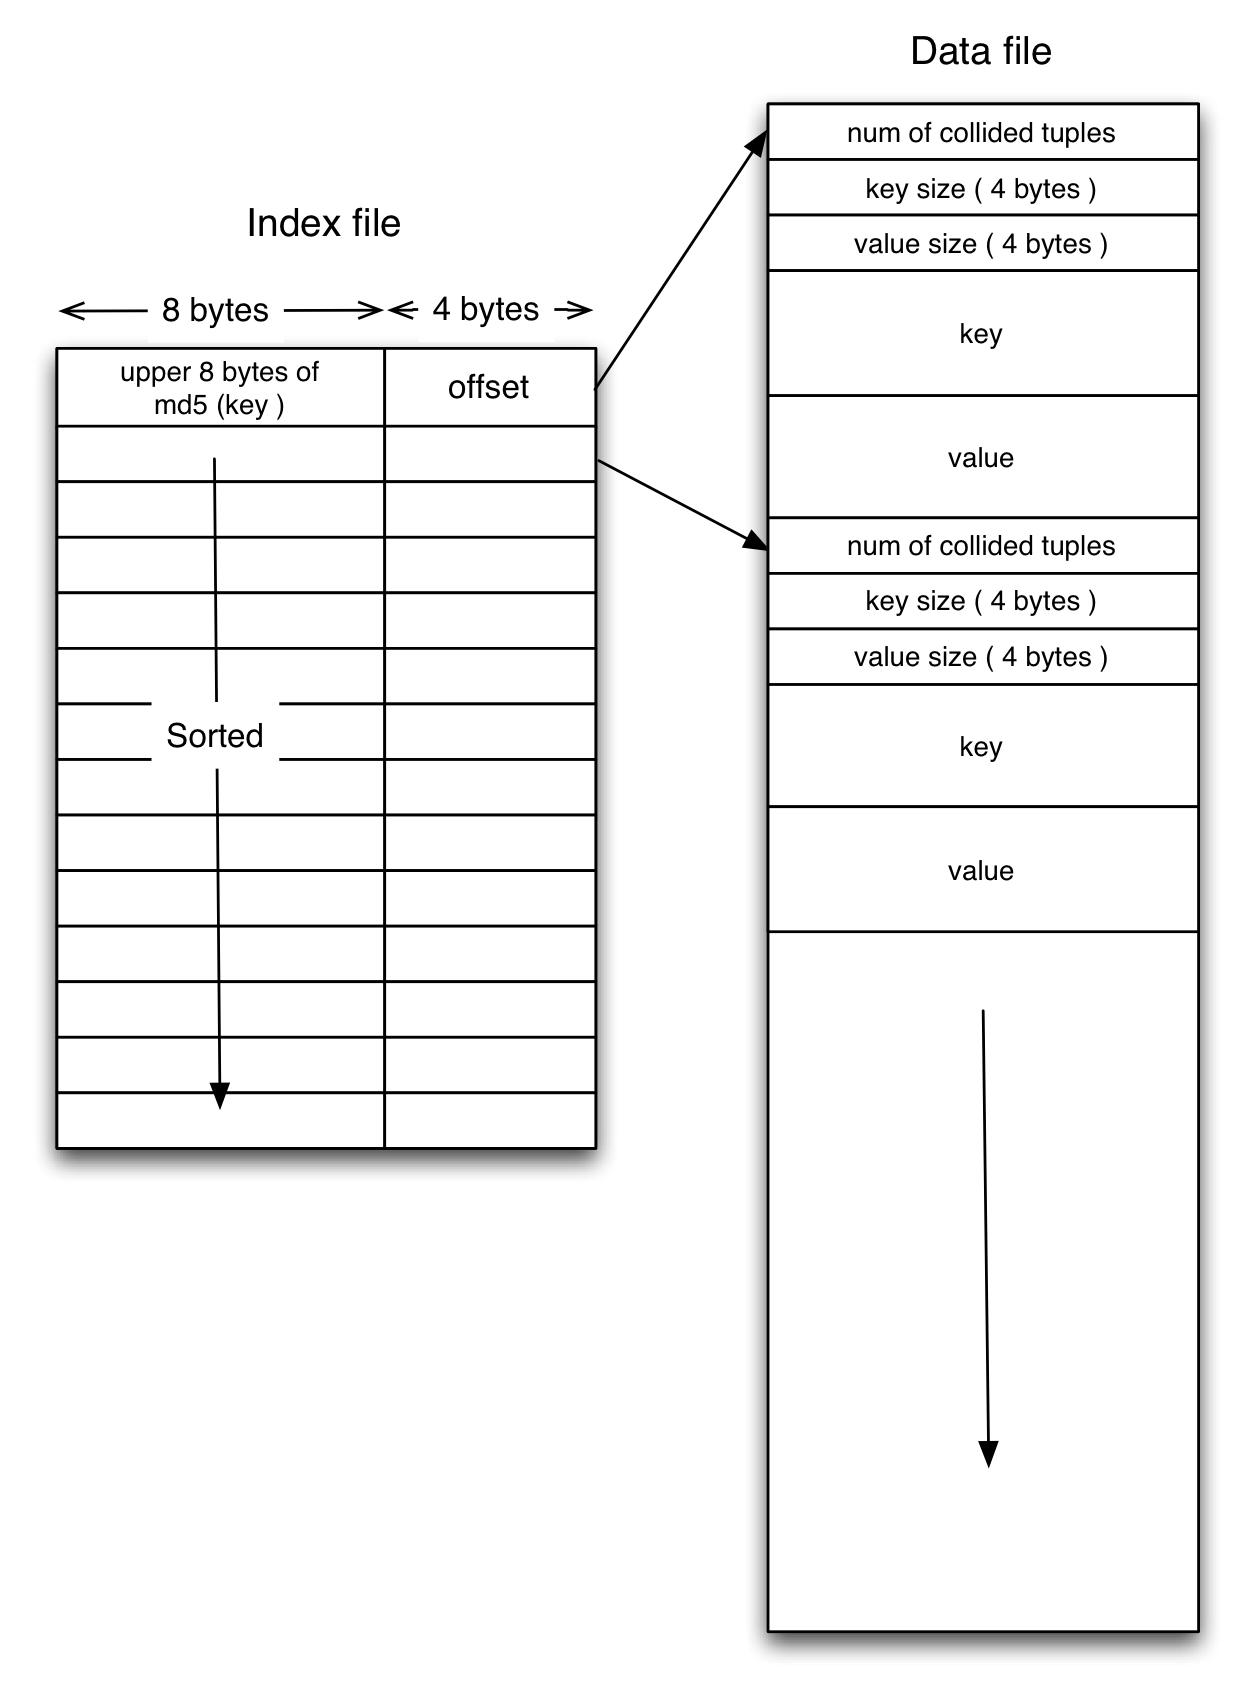
\includegraphics[scale=0.50]{storage_format.png}
\end{center}

We split our data into multiple chunks where every chunk is a pair of data and index file. There are two reasons to split the data into multiple chunks - (a) parallelism achieved on the Hadoop side (b) limitation of Java to memory map files upto a maximum of 2 GB. We build multiple chunks for every partition-replica bucket. Building chunks at this granularity helps with rebalancing, more about which we will explain in the following subsections. We have set a standard naming convention for all our chunk files. It follows the pattern $<partition\,id>\_<replica\,type>\_<chunk\,id>.data|index$, where $partition\,id$ is the id of the primary partition and $replica\,type$ is a number between 0 to `replication factor'-1. Once a key hashes to a particular node, we classify it into the correct $partition\,id$ + $replica\,type$ bucket. We then take all the tuples in this bucket and split it up into multiple smaller chunks. The following table shows the various bucket names ( where every bucket will contain multiple chunks and each chunk will in turn contain an index and data file ) for a store with consistent hash routing and replication factor 2. This assumes that the cluster has the same partition ring topology as shown in Figure 2. This bucket granularity was definitely not present in our first iteration since we have initially started by defining a bucket to be only on a per node basis ( i.e. multiple chunks stored on a node with no knowledge about partitions ). Over time we realized that breaking up the bucket into smaller granularity would help rebalancing. We will describe this in more details in Section 4.3.2. 

\begin{center}
    \begin{tabular}{ | c | c | }
    \hline
    Node & Chunk files \\ \hline
   Node 0 &  0\_0, 5\_0, 4\_1, 7\_1 \\
   Node 1 &   1\_0, 3\_0, 7\_0, 0\_1, 2\_1, 6\_1 \\
   Node 2 &    2\_0, 4\_0, 6\_0, 1\_1, 3\_1, 5\_1  \\
\hline
    \end{tabular}
\end{center}


The index file is a compact structure containing sorted upper 8 bytes of the MD5 of the key followed by the 4 byte offset of the corresponding value in the data file. The primary reason to go for this simple sorted structure, in comparison to various previous complicated page aware structures described in literature, was to keep the build process simple. Since we wanted to leverage Hadoop for our index construction we had to face the inherent limitation that generally mapper and reducer tasks do not have much memory. Building complicated structures then would require us to explore various fancy external tree building functions thereby making the process very error prone. Preliminary tests also showed that the index files were generally order of magnitude smaller than the data files. Hence we could safely assume that they would fit into page cache easily. 

We had initially started by using all 16 bytes of the MD5 of the key in the index file. But over time as we started on-boarding various new stores we started getting performance problem. This was happening because having lots of stores was resulting in stamping on each others pages in the page cache. To alleviate this problem we needed to cut down on the amount of data being memory mapped. This could be achieved by cutting down on the number of bytes of the MD5 of the key and accepting collisions in the data file. Then the next important question was, how many bytes do we trim down the key to? This can easily be mapped to birthday paradox which says that if we want to retrieve $n$ random integers from a uniform distribution of range $[1, x]$, the probability that at least 2 numbers are the same is  $1 - e^{(-n(n-1)/2x})$. Mapping this to our read-only stores scenario, say our read-only store is saving recommendation for our 120 million member user base. So $n$ = 120 million and $x$ = $2^{128}$ ( 16 bytes ) gives us a probability of collision to be close to 0. Decreasing this to say 4 bytes ( i.e. 32 bit ) gave a high probability of $1 - e^{\frac{(-120*10^{6} * ( 120*10^{6} - 1)}{2^{32}}} \sim 1$. But if we instead cut it by half to 8 bytes ( i.e. 64 bits ) we get a very low probability of $1 - e^{\frac{(-120*10^{6} * (120*10^{6} - 1)} { 2^{64}}} \sim 2.0000 * e^{-04}$. The probability of more than one collision is even smaller. In conclusion, we managed to save a lot of space from the page cache but now had to (a) save the keys in the data file to use for lookups (b) take care of rare collisions.  

The data file is similarly a very highly packed structure where we store the number of collided tuples followed by a set of collided $key\,size, value\,size, key, value$ list. The important thing to remember here is that we store the raw key bytes instead of the MD5-ed key bytes in order to do a comparison during reads. 

\subsubsection{Construction of chunk files}

Construction of the chunk files for all nodes is a single MapReduce job. The following is a pseudo-code representation of the complete job. 


The Hadoop-based store builder is actually substantially simpler than the single-process builder as it leans heavily on Hadoop’s native capabilities to do its work. The store building processes proceeds as follows. An user-extensible Mapper extracts keys from the source data. This mapper can be parametrized to work with different InputFormats, and provides hooks to allow custom ways to construct the key and value from the data. A custom Hadoop Partitioner then applies the Voldemort consistent hashing function to the keys, and assigns all keys mapped to a given node and chunk to a single reduce task. The shuffle phase of the map/reduce copies all values with the same destination node and chunk to the same reduce task. Thus each of the reduce tasks will create one .index and .data file for a given chunk on a particular node; and as a result the number of chunks specified in the configuration acts as a parameter to control the parallelism of the build. These values are then sorted by Hadoop in order to group them by key for reduce. Each reduce task copies the key/value pairs it is given into a pair of .index and .data files in sorted order to build its store chunk.

\subsubsection{Search}

Having a fixed space requirement for every key ( 12 bytes ) makes it easy to do lookups with no internal pointers required within the index files. For example to find the data location of the $i$th element in the sorted index is a simple jump to the offset 12 * $i$ + 8 from where we can read the offset to the data file.

A lookup in the store proceeds as follows:

Calculate the MD5 of the key
The first 4 bytes of this md5, modulo the number of chunks, is the chunk number to search in
Do a binary search for the key md5 in that chunk’s .index file to get the position of the value in the data file
Finally read the appropriate number of bytes for the value from the data file starting at the given position
The code for this storage engine is quite simple, only a few hundred lines, with the distribution and fault tolerance–the hard problems–being provided by the rest of Voldemort.

Binary search is not a very efficient algorithm for finding the location of the data. Most of the time this is not important since the index is in memory and so data access time dominates, but there are two cases that could be improved. The first is the case where all data and index fit entirely in memory. With very small keys, a chunk might have an index with, say, 100 million entries, which means a binary search does 27 key reads and comparisons and a single data read. In this case the cost of the search will dominate. Another suboptimal case is when we have an entirely uncached index. We explicitly transfer index files last in the data deployment to avoid this case, however in the case of rolling back to a previous index version it is unavoidable. To page the 100 million entry index for a chunk into memory will require 500k page faults no matter what the structure is. However it would be desirable to minimize the maximum number of page faults incurred on a given request to minimize the variance of the request time. In this case a page-organized tree, where each parent had 204 20 byte children, could do only log\_204(100 million) = 4.5 page faults in the worst case and would be superior.

To resolve these cases we are working on an improved search algorithm which takes into account the uniformity of the key distribution, whch results from the fact that MD5 is (somewhat) cryptographically secure and so its keys are uniformly distributed. Rather than always beginning with a comparison to the middle entry such an algorithm would use the uniformity of the key distribution to compute the expected quantile of the key being looked up attempting to jump immediately to the correct location. If we can get a reliable implementation this promises to greatly improve the number of both page faults and comparisons needed in these corner cases.



\subsection{Versioning of data}
Helps with rollbacks


\subsection{Complete data cycle}

Diagram with our complete pipeline including Azkaban...

\subsubsection{Schema changes}


\subsubsection{Rebalancing}


\subsubsection{Compression}
\begin{itemize}
	\item Both at row level and copying level
\end{itemize}



\section{Experience}
LinkedIn has been successfully been using Voldemort read-only stores for the past 2 years. It has become an integral part of our data-cycle and has 

\begin{itemize}
	\item Random dataset
- Run on member\_id to uniform key of 1024 bytes
- The time to completion increases linearly with the size of the dataset and is comparable between different types of data

a) Single node - Increase in size of dataset - 1GB, 2GB, 4GB, 8GB, 16GB, 32GB, 64GB, 128GB 
       [ Metric 1 ] Time to build
       [ Metric 2 ] Time to query ( Median, 99th ) - YCSB - 100 million keys - Uniform, Zipfian 

b) 16 node - Increase in size of dataset ( 128 GB, 256 GB, 512 GB, 1TB )
      [ Metric 1 ] Time to build
      [ Metric 2 ] Time to query ( Median, 99th ) - YCSB - 100 million keys - Uniform, Zipfian 

	\item PYMK dataset
	a) 16 node 
       - Time to build
       - Time to query ( Median, 99th ) - YCSB - 100 million keys - Uniform, Zipfian 

	\item Browsemaps dataset
	a) 16 node
	   - Time to build
	   - Time to query ( Median, 99th )
\end{itemize}


\section{Conclusion / Future Work}

MPH \cite{External Perfect Hashing for Very Large Key Sets}, Incremental pushes ( not much use for us as of now since recommendations are floats are they change completely ), Push only one replica

\acks

\bibliographystyle{eurosys}

\bibliography{linkedin}    


\end{document}

